\documentclass[10pt]{article}

\usepackage[margin=0.72in]{geometry}
\usepackage{graphicx}
\usepackage{booktabs}
\usepackage{array}
\usepackage{tikz}
\usetikzlibrary{arrows.meta,positioning}
\usepackage{xcolor}
\usepackage{hyperref}
\usepackage{caption}
\usepackage{float}
\usepackage{amsmath}
\usepackage{amssymb}
\usepackage{enumitem}
\usepackage[section]{placeins}

\hypersetup{colorlinks=true,linkcolor=blue,urlcolor=blue,citecolor=blue}
\setlist{nosep,leftmargin=*}
\captionsetup{font=small,labelfont=bf}

\definecolor{boxblue}{RGB}{221,235,247}
\definecolor{boxgreen}{RGB}{226,239,218}
\definecolor{boxorange}{RGB}{252,228,214}
\definecolor{boxgray}{RGB}{242,242,242}

\title{\vspace{-1.2cm}\textbf{Hexadecimal Image Recognition}\\[-1pt]
\large A Compact Vision Recognizer for Hex-to-Decimal Conversion:\\
Design, Architecture Ablation, Generalization Study, and Deployment}
\author{Sajjad Shahali}
\date{July 2026}

\begin{document}
\maketitle
\vspace{-0.8cm}

\begin{figure}[H]
    \centering
    
\includegraphics[width=0.83\textwidth]{figures/hex_samples_grid.png}
    \caption{Test-set samples spanning font, scale, placement, contrast, and noise
    variation. Each image contains a one-to-three digit hexadecimal literal.}
    \label{fig:samples}
\end{figure}

\begin{abstract}
\noindent
This report presents a small vision recognizer that reads an image of a hexadecimal
literal and returns its decimal value, together with the reasoning behind every
design choice made along the way. The system comprises a synthetic, labeled image
corpus; three architecturally distinct recognizers trained from identical data for a
controlled comparison; a designed (not implemented) reinforcement-learning alignment
stage with a shaped reward function; and a REST deployment. The headline result is not
simply an accuracy number but a reliability finding: one architecture reaches the
highest single-run accuracy, yet only a second, self-attention-based architecture
converges consistently across repeated training runs, and it is that second
architecture which is deployed. Its selected seed-45 checkpoint reaches 96.50\% exact-match
accuracy on 400 held-out images with 607K parameters and roughly one millisecond of
GPU inference latency. Further experiments quantify seed sensitivity, out-of-distribution
degradation, and a rotation-recovery pipeline that lifts sideways/upside-down accuracy
from 6.00\% to 80.00\%.
\end{abstract}

% ============================================================
\section{Problem Framing and Design Philosophy}
% ============================================================

The task is to map an image containing a value between \texttt{0x0} and \texttt{0xfff}
to the corresponding decimal integer. Although the assignment brief refers to a
Vision-Language Model, this is a closed, sixteen-symbol vocabulary recognition problem
with a deterministic downstream conversion -- a case where a compact convolutional
recognizer is the better-fitted tool than a large pretrained vision-language stack. The
system therefore separates two concerns deliberately: a learned model reads the glyphs
(e.g.\ \texttt{0x1a4}), and a fixed, non-learned rule converts the literal to its integer
value (420). This separation keeps the one genuinely hard sub-problem -- visual
character recognition under font, scale, and noise variation -- isolated from the trivial
one, and makes the two failure modes easy to tell apart during evaluation.

\begin{figure}[H]
\centering
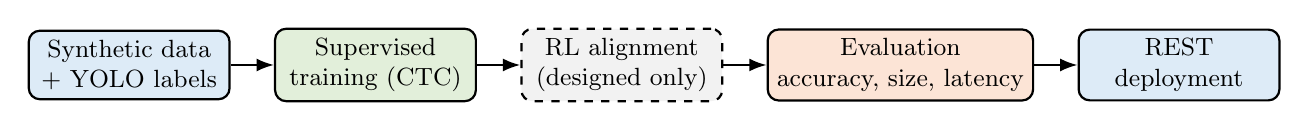
\begin{tikzpicture}[
    node distance=0.55cm,
    stage/.style={rectangle,rounded corners,draw,thick,minimum height=0.85cm,
                  minimum width=2.55cm,align=center,font=\small},
    arrow/.style={-{Latex[length=2.2mm]},thick}
]
    \node[stage,fill=boxblue] (data) {Synthetic data\\+ YOLO labels};
    \node[stage,fill=boxgreen,right=of data] (sft) {Supervised\\training (CTC)};
    \node[stage,fill=boxgray,dashed,right=of sft] (rl) {RL alignment\\(designed only)};
    \node[stage,fill=boxorange,right=of rl] (eval) {Evaluation\\accuracy, size, latency};
    \node[stage,fill=boxblue,right=of eval] (api) {REST\\deployment};
    \draw[arrow] (data)--(sft);
    \draw[arrow] (sft)--(rl);
    \draw[arrow] (rl)--(eval);
    \draw[arrow] (eval)--(api);
\end{tikzpicture}
\caption{End-to-end lifecycle. Reinforcement learning is a designed, optional
alignment stage (Section~\ref{sec:rl}); the deployed recognizer is trained with
supervised CTC loss only.}
\label{fig:lifecycle}
\end{figure}

Reinforcement learning is not required for this deterministic task -- supervised
training with a CTC loss already optimizes the exact objective end to end -- so it is
specified in full as a design exercise (Section~\ref{sec:rl}) rather than executed,
targeting a hypothetical future variant where the model generates free-form text
instead of a fixed-vocabulary sequence.

% ============================================================
\section{Dataset}
% ============================================================

The corpus is generated synthetically rather than sourced, which makes every property
of the training distribution a controllable design decision rather than an accident of
data collection. 3{,}800 labeled images were rendered and split as shown in
Table~\ref{tab:data}, with a near-balanced spread across one-, two-, and three-digit
values -- a natural byproduct of sampling values uniformly by digit count rather than an
explicit stratification step.

\begin{table}[H]
\centering
\begin{tabular}{@{}lrrl@{}}
\toprule
\textbf{Split} & \textbf{Images} & \textbf{Share} & \textbf{Purpose} \\
\midrule
Train      & 3,000 & 78.9\% & Model optimization \\
Validation &   400 & 10.5\% & Checkpoint selection \\
Test       &   400 & 10.5\% & Final held-out evaluation \\
\midrule
Total      & 3,800 & 100\% & \\
\bottomrule
\end{tabular}
\qquad
\begin{tabular}{@{}lr@{}}
\toprule
\textbf{Hex digits} & \textbf{Count} \\
\midrule
1 (\texttt{0x0}--\texttt{0xf})   & 1,250 \\
2 (\texttt{0x10}--\texttt{0xff}) & 1,277 \\
3 (\texttt{0x100}--\texttt{0xfff}) & 1,273 \\
\midrule
Total & 3,800 \\
\bottomrule
\end{tabular}
\caption{Split allocation and digit-length distribution. The underlying value space
has only 4{,}096 possible literals, smaller than the training split itself, so values
necessarily repeat across splits under independently rendered images -- expected and
correct behavior for a closed-set recognition task, not a leak.}
\label{tab:data}
\end{table}

Five robustness controls were injected specifically to prevent the model from
memorizing pixel layouts rather than learning glyph shape: a pool of twelve fonts,
size and position jitter, small-angle rotation ($\pm 8^{\circ}$, simulating imperfect
photo alignment), foreground/background color variation, and Gaussian pixel noise
(Table~\ref{tab:knobs}). Every rendered glyph -- including the literal \texttt{0} and
\texttt{x} of the prefix -- receives an exact bounding box derived from the renderer's
own placement geometry, satisfying the assignment's labeling requirement even though the
sequence recognizer itself does not consume per-character boxes (Figure~\ref{fig:bbox}).

\begin{table}[H]
\centering
\begin{tabular}{@{}lp{5.4cm}@{}}
\toprule
\textbf{Control} & \textbf{Failure mode it targets} \\
\midrule
Font variety (12 fonts) & Memorizing one font's fixed pixel pattern \\
Size jitter & Variable apparent camera distance \\
Position jitter & A fixed spatial prior on character location \\
Small-angle rotation & Imperfectly aligned capture \\
Color/noise variation & Lighting and sensor variation \\
\bottomrule
\end{tabular}
\caption{Data augmentation controls and the failure mode each targets.}
\label{tab:knobs}
\end{table}

\begin{figure}[H]
    \centering
    
\includegraphics[width=0.42\textwidth]{../logs/plots/bbox_sanity_check.png}
    \caption{Character-level bounding boxes on a real sample, confirming label
    alignment against the rendered glyphs.}
    \label{fig:bbox}
\end{figure}

% ============================================================
\section{Recognizer Architectures}
% ============================================================

Rather than commit to a single architecture and cite literature to justify it after the
fact, three sequence-modeling heads were built on top of one shared convolutional
feature extractor and evaluated under identical data and training budget
(Table~\ref{tab:models}). Sharing the visual front end means any accuracy or latency
difference between the three is attributable to the sequence head, not to different
learned features -- an actual controlled ablation rather than a single choice presented
as though it were obviously correct.

\begin{table}[H]
\centering
\begin{tabular}{@{}lp{8.6cm}r@{}}
\toprule
\textbf{Architecture} & \textbf{Sequence head} & \textbf{Parameters} \\
\midrule
CRNN & One-layer bidirectional GRU; a strong inductive bias for ordered
     sequences \cite{liu2022} & 542,226 \\
FCN & Three dilated 1-D convolutions (dilations 1, 2, 4), fully parallel,
    no recurrence \cite{yousef2018,coquenet2020} & 490,386 \\
ConvAttn & Two-layer, four-head self-attention encoder with positional encoding
         \cite{hernandezdiaz2021} & 606,738 \\
\bottomrule
\end{tabular}
\caption{The three candidate recognizers. All three share an identical convolutional
stem and CTC output layer, differing only in how the character sequence is modeled.}
\label{tab:models}
\end{table}

\subsection{Problem formulation}

Let an input image be
$\mathbf{x}\in\mathbb{R}^{1\times32\times128}$ and let the target transcription be
$\mathbf{y}=(y_1,\ldots,y_U)$, where
$y_u\in\mathcal{V}=\{\texttt{0},\ldots,\texttt{9},\texttt{a},\ldots,\texttt{f},
\texttt{x}\}$ and $U\in\{3,4,5\}$. The recognizer produces a distribution over
$|\mathcal{V}|+1=18$ classes at each of $T=32$ horizontal timesteps; the extra class
is the CTC blank. The learned task is therefore image-to-sequence transcription.
Hexadecimal-to-decimal conversion is deliberately not learned:
\[
    \hat{d} = \operatorname{int}(\hat{\mathbf{y}},16).
\]
This decomposition prevents a correct visual transcription from being confused with a
conversion error and guarantees mathematically exact conversion whenever the
transcription is correct.

\subsection{Shared convolutional feature extractor}

The CNN converts spatial pixels into a left-to-right sequence. Width is reduced only
twice, from 128 to 32, while height is progressively collapsed to one row. Each of the
32 remaining columns becomes one sequence timestep with a 128-dimensional descriptor.

\begin{table}[H]
\centering
\small
\begin{tabular}{@{}lllr@{}}
\toprule
\textbf{Stage} & \textbf{Operation} & \textbf{Output shape} & \textbf{Role} \\
\midrule
Input & grayscale normalization & $1\times32\times128$ & pixel input \\
Block 1 & Conv $3\times3$, ReLU, Pool $2\times2$ &
    $32\times16\times64$ & edges/strokes \\
Block 2 & Conv $3\times3$, ReLU, Pool $2\times2$ &
    $64\times8\times32$ & glyph parts \\
Block 3 & Conv $3\times3$, norm, Pool $2\times1$ &
    $128\times4\times32$ & preserve sequence width \\
Block 4 & Conv $3\times3$, norm, Pool $2\times1$ &
    $128\times2\times32$ & vertical compression \\
Collapse & Conv $2\times3$, norm, ReLU &
    $128\times1\times32$ & 32-step sequence \\
\bottomrule
\end{tabular}
\caption{Shared CNN stem. Shapes omit the batch dimension. The deliberate asymmetric
pooling preserves horizontal reading order while collapsing height.}
\label{tab:cnn-stem}
\end{table}

This design is efficient for upright text but also explains a later result: a
height-collapsed representation is poorly suited to 90-degree text, where characters
are arranged vertically. That limitation motivates the separate orientation classifier
in Section~\ref{sec:generalization}.

\subsection{CRNN: bidirectional recurrent sequence modeling}

The CRNN follows the standard convolutional-recurrent OCR pattern
\cite{liu2022}. After the CNN, the feature at column $t$ is
$\mathbf{h}_t\in\mathbb{R}^{128}$. A forward GRU processes columns from left to right
and a backward GRU processes them from right to left:
\[
 \overrightarrow{\mathbf{s}}_t =
 \operatorname{GRU}_f(\mathbf{h}_t,\overrightarrow{\mathbf{s}}_{t-1}),\qquad
 \overleftarrow{\mathbf{s}}_t =
 \operatorname{GRU}_b(\mathbf{h}_t,\overleftarrow{\mathbf{s}}_{t+1}).
\]
Their states are concatenated and projected to character logits,
\[
 \mathbf{z}_t=W[\overrightarrow{\mathbf{s}}_t;
 \overleftarrow{\mathbf{s}}_t]+\mathbf{b}.
\]
Bidirectionality is useful because an ambiguous local stroke can be interpreted using
characters on both sides. The ordered recurrent state is a strong inductive bias for
text, but timesteps are processed sequentially within each direction and the training
results show sensitivity to initialization.

\subsection{FCN: dilated temporal convolutions}

The FCN removes recurrence. The CNN sequence is transposed to
$B\times128\times32$ and passed through three width-preserving Conv1d layers with
dilations 1, 2, and 4. With kernel size three, the stack has a 15-timestep receptive
field (radius seven) while retaining all 32 output positions. Thus
\[
 \mathbf{H}^{(\ell+1)} =
 \operatorname{ReLU}\!\left(
 \operatorname{Norm}\!\left(
 \operatorname{Conv1D}_{d_\ell}(\mathbf{H}^{(\ell)})
 \right)\right),\quad d_\ell\in\{1,2,4\}.
\]
All positions can be evaluated in parallel, and this variant has the fewest parameters.
Its limitation is that context is fixed by the receptive field rather than selected
dynamically. In this experiment it is also the least stable architecture across seeds,
showing that theoretical parallelism does not guarantee easier optimization.

\subsection{ConvAttn: global self-attention}

ConvAttn adds sinusoidal position encodings to the CNN sequence and applies two
Transformer encoder layers with four attention heads. For one head,
\[
 \operatorname{Attention}(Q,K,V)=
 \operatorname{softmax}\!\left(\frac{QK^\top}{\sqrt{d_k}}\right)V.
\]
Every output position can therefore use evidence from every image column in one layer,
unlike the FCN's fixed local context or the GRU's recurrent state. Position encodings
remain necessary because self-attention alone is permutation invariant. Each encoder
layer also contains a 256-dimensional feed-forward block, residual connections, layer
normalization, and dropout. This head is the largest and slowest of the three, but its
five-seed variance is dramatically lower; that reliability, rather than a claim that
self-attention always dominates recurrence, motivates deployment.

\subsection{CTC objective and decoding}

Character boxes are not used by the recognizer. CTC marginalizes over all timestep
alignments that collapse to the target string. If $\mathcal{B}$ removes blanks and
merges adjacent repeated labels, the loss is
\[
\mathcal{L}_{\mathrm{CTC}} =
-\log \sum_{\boldsymbol{\pi}\in\mathcal{B}^{-1}(\mathbf{y})}
\prod_{t=1}^{T}p_t(\pi_t\mid\mathbf{x}).
\]
This permits training from image/string pairs without assigning each character to a
specific column. At inference, greedy decoding takes the most probable class per
timestep, merges repeats, and removes blanks. It is fast and adequate for this small
vocabulary, but it explains the observed failure mode in which adjacent repeated
characters are occasionally collapsed.

\begin{figure}[H]
\centering
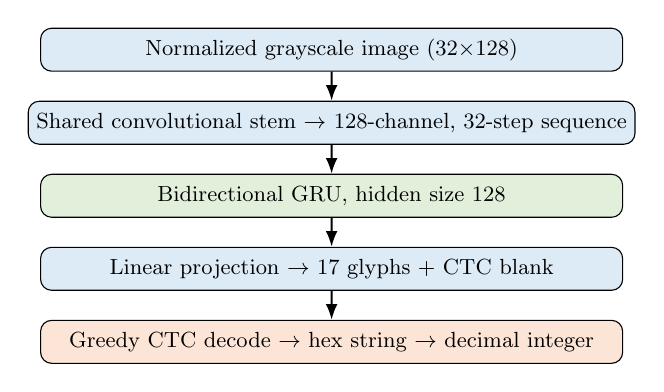
\begin{tikzpicture}[scale=0.88,transform shape,
    node distance=0.42cm,
    block/.style={rectangle,draw,rounded corners,fill=boxblue,minimum width=8.4cm,
                  minimum height=0.62cm,font=\small,align=center},
    arrow/.style={-{Latex[length=2mm]},thick}
]
    \node[block] (in) {Normalized grayscale image ($32{\times}128$)};
    \node[block,below=of in] (cnn) {Shared convolutional stem $\rightarrow$
        128-channel, 32-step sequence};
    \node[block,below=of cnn,fill=boxgreen] (rnn) {Bidirectional GRU, hidden size 128};
    \node[block,below=of rnn] (out) {Linear projection $\rightarrow$ 17 glyphs + CTC
        blank};
    \node[block,below=of out,fill=boxorange] (decode) {Greedy CTC decode
    $\rightarrow$ hex string $\rightarrow$ decimal integer};
    \draw[arrow] (in)--(cnn);
    \draw[arrow] (cnn)--(rnn);
    \draw[arrow] (rnn)--(out);
    \draw[arrow] (out)--(decode);
\end{tikzpicture}
\caption{CRNN reference architecture. Connectionist Temporal Classification (CTC)
learns character alignment without needing character-level box supervision. ConvAttn
replaces the recurrent block with a self-attention encoder; FCN replaces it with
dilated convolutions.}
\label{fig:crnn}
\end{figure}

All three were trained from scratch, with Adam, an initial learning rate of $10^{-3}$
under cosine decay, batch size 64, gradient clipping, and up to 80 epochs with early
stopping on validation exact-match accuracy. No pretrained backbone and no
reinforcement-learning signal are used at this stage -- the CTC loss on the labeled
transcription is the entire supervisory signal.

\begin{table}[H]
\centering
\small
\begin{tabular}{@{}ll@{}}
\toprule
\textbf{Training item} & \textbf{Configuration} \\
\midrule
Optimizer & Adam \\
Initial learning rate & $10^{-3}$ \\
Schedule & cosine annealing \\
Batch size & 64 \\
Maximum epochs & 80 \\
Early-stopping patience & 12 epochs \\
Gradient clipping & maximum norm 5.0 \\
Model selection & highest validation exact-match accuracy \\
Reliability seeds & 42, 43, 44, 45, 46 \\
Hardware & NVIDIA RTX 5070 Ti, CUDA 12.8 \\
\bottomrule
\end{tabular}
\caption{Training protocol shared by the controlled architecture experiments.}
\label{tab:training-config}
\end{table}

% ============================================================
\section{Evaluation and Architecture Comparison}
% ============================================================

\subsection{Evaluation protocol}

Four complementary measurements are used. Hex exact match is
$N^{-1}\sum_i\mathbf{1}[\hat{y}_i=y_i]$ and directly measures transcription.
Decimal exact match compares the deterministically parsed values and is the end-user
task metric. Character accuracy is a position-wise diagnostic divided by the longer of
prediction and target; it is not presented as standardized edit-distance CER. Model
footprint is reported as trainable parameter count and serialized checkpoint size.
Latency is measured using 100 synchronized batch-1 GPU passes after 15 warm-up passes,
matching the single-request serving pattern rather than dividing batched throughput by
batch size.

\begin{table}[H]
\centering
\small
\begin{tabular}{@{}lrrrrrr@{}}
\toprule
\textbf{Model} & \textbf{Hex EM} & \textbf{Char acc.} & \textbf{Params}
& \textbf{Size} & \textbf{Mean} & \textbf{p95} \\
 & & & & \textbf{(MB)} & \multicolumn{2}{c}{\textbf{latency (ms)}} \\
\midrule
CRNN      & 96.50\% & 99.04\% & 542K & 2.082 & \textbf{0.663} & \textbf{0.764} \\
FCN       & 87.00\% & 96.35\% & \textbf{490K} & \textbf{1.892} & 0.707 & 0.832 \\
ConvAttn & 94.50\% & 98.28\% & 607K & 2.367 & 1.015 & 1.148 \\
\bottomrule
\end{tabular}
\caption{Held-out test-set results ($n=400$) for the controlled seed-42 comparison.
The selected ConvAttn seed-45 deployment checkpoint reaches 96.50\% hex/decimal exact
match and 99.11\% character accuracy. Latency is measured as 100 synchronized,
single-image GPU forward
passes after warm-up -- the same request pattern the deployed API serves.}
\label{tab:results}
\end{table}

\begin{figure}[H]
    \centering
    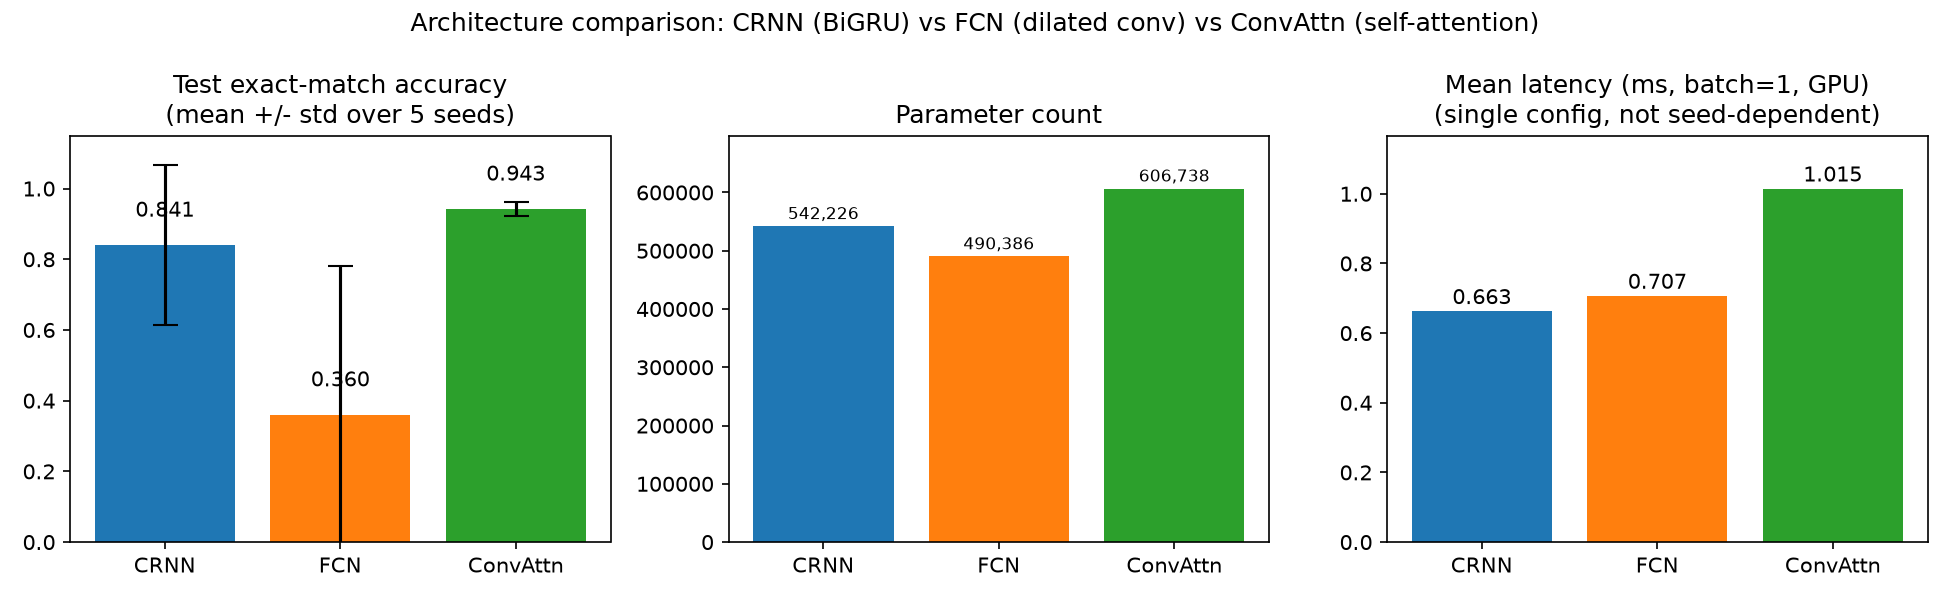
\includegraphics[width=\textwidth]{../logs/plots/architecture_comparison.png}
    \caption{Architecture trade-offs. Test exact-match accuracy is the mean
    $\pm$ standard deviation across five seeds; parameter count and synchronized
    batch-1 GPU latency are fixed architecture properties. ConvAttn is slightly
    larger and slower, but its training outcome is substantially more reliable.}
    \label{fig:architecture-comparison}
\end{figure}

Read on its own, this table would suggest CRNN as the obvious choice: it leads on
accuracy and latency both. That conclusion does not survive repeated training, which is
the subject of the next section and the actual basis for the deployment decision.

Error analysis on CRNN's 14 test-set mismatches found that every one remained a
well-formed, valid hexadecimal literal -- none were malformed output. The dominant
failure pattern is adjacent or repeated identical glyphs being dropped
(e.g.\ \texttt{0x77f}$\to$\texttt{0x7f}), a direct consequence of the CTC decoding rule
that collapses repeated symbols. Accuracy also degrades mildly with value length:
99.29\% for one-digit values, 95.56\% for two digits, 94.40\% for three digits --
consistent with longer sequences giving the repeat-collapse rule more opportunities to
misfire, not with any single glyph being systematically harder to read.

% ============================================================
\section{Generalization Study}
\label{sec:generalization}
% ============================================================

A single test-set number, from a single trained checkpoint, is a narrow claim. Four
follow-up experiments were run specifically to find out how narrow.

\subsection{Seed reliability -- the central finding}

Each architecture was retrained five times from different random seeds under identical
data and hyperparameters (Figure~\ref{fig:seeds}, Table~\ref{tab:seeds}). CRNN and FCN
both swing between near-collapse and their best-case accuracy depending on
initialization alone; ConvAttn does not.

\begin{figure}[H]
    \centering
    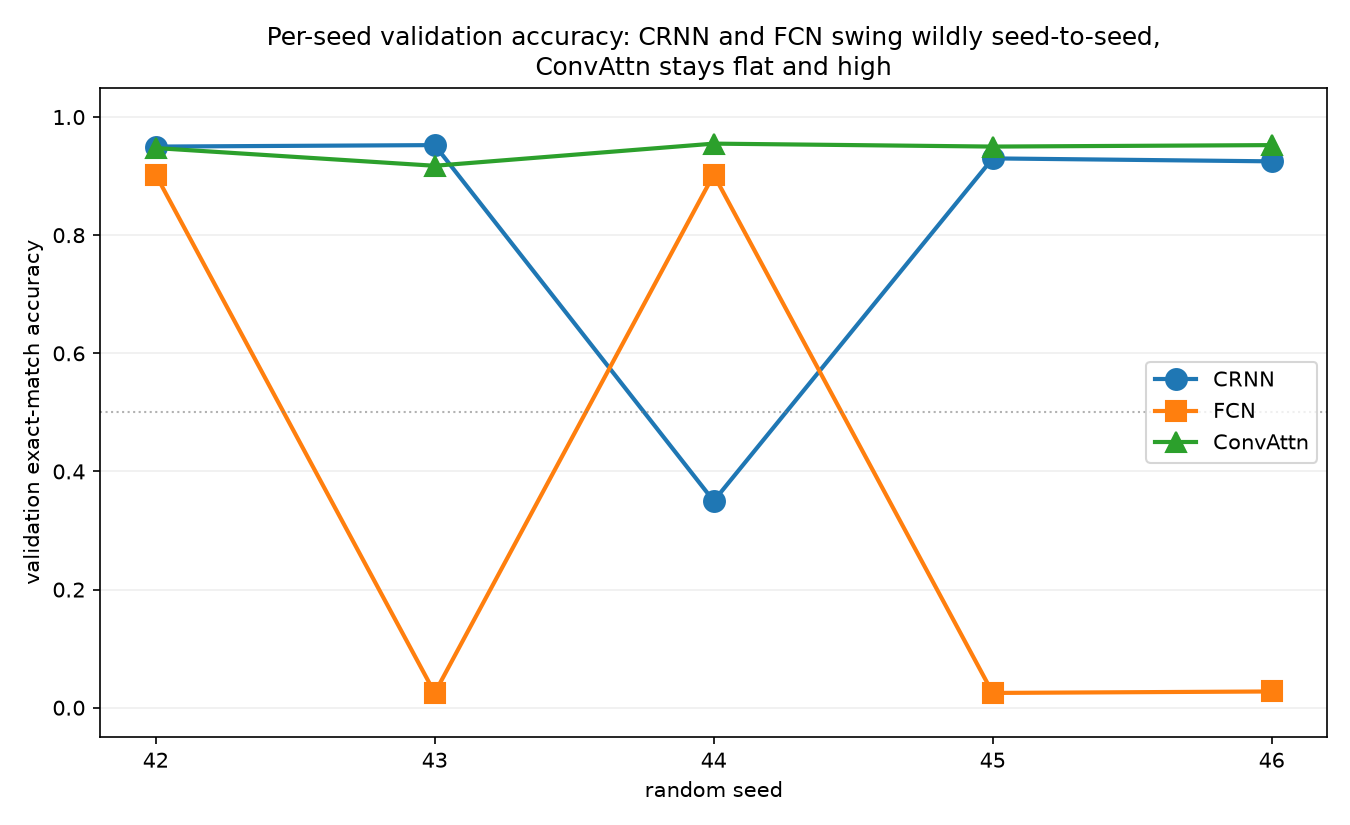
\includegraphics[width=0.72\textwidth]{../logs/plots/per_seed_accuracy_lines.png}
    \caption{Best validation exact-match accuracy across five random seeds. CRNN and
    FCN are highly seed-sensitive; ConvAttn stays in a narrow, high-accuracy band on
    every seed tried.}
    \label{fig:seeds}
\end{figure}

\begin{table}[H]
\centering
\begin{tabular}{@{}lrrrr@{}}
\toprule
\textbf{Architecture} & \textbf{Mean} & \textbf{Std.\ dev.} & \textbf{Min} & \textbf{Max} \\
\midrule
CRNN      & 82.15\% & 23.6 pts & 35.00\% & 95.25\% \\
FCN       & 37.65\% & 43.0 pts &  2.50\% & 90.25\% \\
ConvAttn  & \textbf{94.45\%} & \textbf{1.4 pts} & \textbf{91.75\%} & 95.50\% \\
\bottomrule
\end{tabular}
\caption{Five-seed validation statistics. CRNN can reach an accuracy essentially tied
with ConvAttn's best case, but only on a favorable seed; ConvAttn reaches that level
on every seed tried.}
\label{tab:seeds}
\end{table}

This is the reason ConvAttn, not CRNN, is deployed despite trailing on
Table~\ref{tab:results}'s single run: a two-point accuracy edge that depends on having
drawn a lucky initialization is not a real advantage for a system meant to be
retrained or refreshed without a human manually re-checking every run. The instability
traces to a specific, diagnosable cause rather than being an unexplained property of
CTC training in general: an earlier design used a square input canvas with a deeper
convolutional stem (to support in-recognizer rotation training, discussed below), and
reverting to the shallower, rectangular canvas measurably improved CRNN's reliability
(mean validation accuracy rising from 55\% to 82\% across the same five seeds), though
not completely. FCN's instability turned out to be independent of that fix and remains
an open issue specific to its dilated-convolution design. Several standard mitigations
-- learning-rate warmup, alternative normalization, a lower learning rate, biased
output-layer initialization -- were tried against the instability and each traded one
failure mode for another rather than resolving it cleanly, which is itself informative:
the instability is a genuine architectural sensitivity, not a tuning oversight with an
easy fix.

\subsection{Rotation robustness}

A natural follow-up question is whether the recognizer generalizes to sideways or
upside-down text, not just the small rotation jitter already in the training
distribution. Training the recognizer directly on 90/180/270-degree rotated images
collapsed accuracy to roughly 20\% -- traced to the convolutional stem's deliberate
compression of image height to a single row, which is correct for horizontal text but
destroys exactly the information needed to distinguish vertically stacked characters.
Rather than redesign the recognizer around a rare case, orientation handling was moved
into a lightweight, independent pre-processing stage: a 60,836-parameter four-way
classifier detects orientation and de-rotates the image before the unmodified,
seed-stable recognizer ever sees it (Table~\ref{tab:rotation}).

\begin{table}[H]
\centering
\begin{tabular}{@{}lr@{}}
\toprule
\textbf{Rotated-image condition} & \textbf{Exact match} \\
\midrule
Recognizer alone, no correction & 6.00\% \\
Orientation classifier (its own task) & 99.00\% \\
Full detect $\to$ de-rotate $\to$ recognize pipeline & \textbf{80.00\%} \\
\bottomrule
\end{tabular}
\caption{Rotation-recovery evaluation using the deployed ConvAttn seed-45 checkpoint
on 300 balanced samples across all four
orientations. Isolating orientation into its own easy sub-task recovers the large
majority of the accuracy a single model would otherwise lose trying to be
simultaneously rotation-invariant and precise.}
\label{tab:rotation}
\end{table}

\subsection{Out-of-distribution robustness}

A harder held-out set with unseen fonts, blur, reduced contrast, and wider rotation was
built to probe generalization beyond the training distribution's specific choices. Test
accuracy drops from 96.50\% in-distribution to 46.75\% out-of-distribution -- a
substantial, disclosed gap rather than a hidden one, and the clearest quantified
direction for future work. It is an expected consequence of training on roughly three
thousand images drawn from a fixed twelve-font pool, not a surprising failure.

\begin{figure}[H]
    \centering
    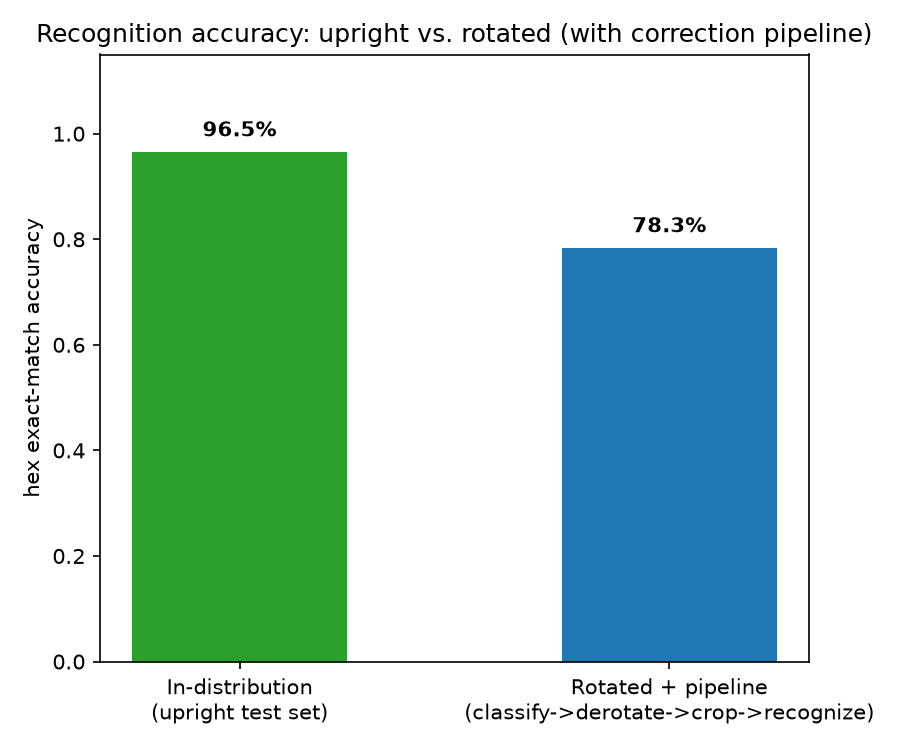
\includegraphics[width=0.68\textwidth]{../logs/plots/generalization_summary.png}
    \caption{ConvAttn generalization as mean $\pm$ population standard deviation
    across seeds 42--46, using the same five checkpoints in every condition.
    The OOD set exposes sensitivity to unseen rendering conditions, while the
    separate orientation-correction stage recovers most of the performance lost
    on sideways and upside-down inputs.}
    \label{fig:generalization-summary}
\end{figure}

\subsection{Hyperparameter search}

A focused search over learning rate and batch size found a configuration that looked
meaningfully better under a short training budget (93.25\% vs. the default's
lower short-budget score), but that advantage disappeared once both configurations were
retrained to full convergence with early stopping -- the untuned default matched or
slightly exceeded the tuned configuration on the final test set. The honest reading is
that a short-budget search optimizes for how quickly a configuration converges, not for
where it ends up, and that the default hyperparameters were already close to as good as
this search could find for the task. The untuned configuration ships.

% ============================================================
\section{Reinforcement Learning Design}
\label{sec:rl}
% ============================================================

Supervised training already optimizes the deployed task directly, so reinforcement
learning is designed here as a forward-looking alignment stage for a hypothetical
generative variant of the model -- one that directly produces a bare decimal integer
rather than a fixed-vocabulary hexadecimal transcription, where exact-match alone would
be too sparse a signal to learn from efficiently. This makes the RL output contract
match the assessment's requested final answer, while the deployed CTC path continues
to transcribe hexadecimal and convert it with a deterministic parser. The proposed
reward remains fully automatic and verifiable, but
decomposes a single pass/fail signal into format, validity, and correctness components
\cite{su2025,liu2026gdpo} (Table~\ref{tab:reward}).

\begin{table}[H]
\centering
\begin{tabular}{@{}lp{3.0cm}p{7.2cm}@{}}
\toprule
\textbf{Component} & \textbf{Reward} & \textbf{Condition} \\
\midrule
Malformed & $-0.5$ & Output is not a bare base-10 integer \\
Format & $+0.2$ & Output follows the decimal-integer syntax \\
Validity & $+0.1$ & Integer is within the task range 0--4095 \\
Exact correctness & $+0.7$ & Decimal output equals ground truth \\
Partial correctness & up to $+0.3c$ & Numeric closeness $c$, capped below exact match \\
\bottomrule
\end{tabular}
\caption{Additive reward for a hypothetical policy that directly emits the requested
decimal answer, ranging from $-0.5$ to $1.0$. Exact correctness alone
outweighs every partial-credit component combined, so the policy cannot learn to
settle for partial credit instead of aiming for the exact value.}
\label{tab:reward}
\end{table}

\begin{figure}[H]
\centering
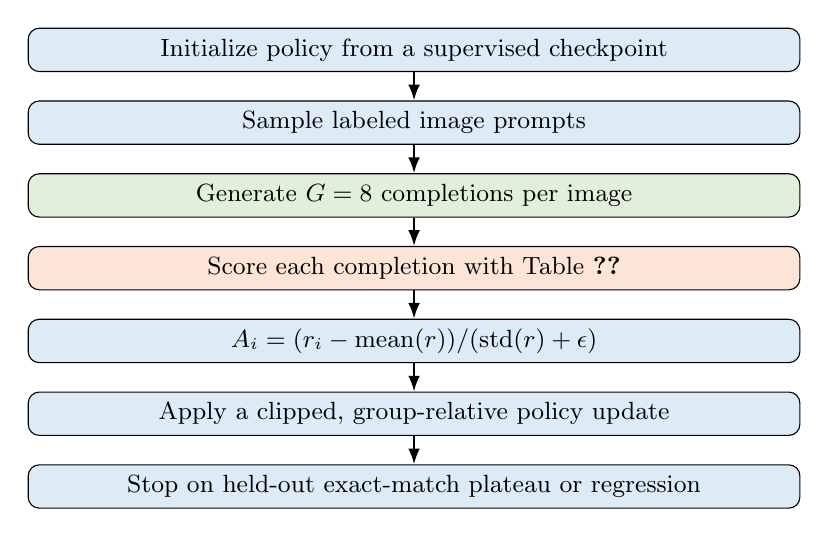
\begin{tikzpicture}[
    node distance=0.36cm,
    block/.style={rectangle,draw,rounded corners,fill=boxblue,minimum width=9.8cm,
                  minimum height=0.55cm,font=\small,align=center},
    arrow/.style={-{Latex[length=2mm]},thick}
]
    \node[block] (init) {Initialize policy from a supervised checkpoint};
    \node[block,below=of init] (sample) {Sample labeled image prompts};
    \node[block,below=of sample,fill=boxgreen] (roll) {Generate $G=8$ completions per image};
    \node[block,below=of roll,fill=boxorange] (score) {Score each completion with Table~\ref{tab:reward}};
    \node[block,below=of score] (adv) {$A_i=(r_i-\operatorname{mean}(r))/(\operatorname{std}(r)+\epsilon)$};
    \node[block,below=of adv] (update) {Apply a clipped, group-relative policy update};
    \node[block,below=of update] (validate) {Stop on held-out exact-match plateau or regression};
    \draw[arrow] (init)--(sample);
    \draw[arrow] (sample)--(roll);
    \draw[arrow] (roll)--(score);
    \draw[arrow] (score)--(adv);
    \draw[arrow] (adv)--(update);
    \draw[arrow] (update)--(validate);
\end{tikzpicture}
\caption{Group-relative policy-optimization loop. Normalizing reward within each
sampled group removes the need for a separately trained critic while preserving
exact-match as the evaluation metric of record.}
\label{fig:grpo}
\end{figure}

The evaluation metric reported at the end of training remains strict exact match, not
the shaped reward -- this keeps the partial-credit terms useful for learning signal
without letting them inflate the headline result.

% ============================================================
\clearpage
\section{Deployment}
% ============================================================

The recognizer is served behind a REST interface with a health-check endpoint and a
single prediction endpoint that accepts an image and returns the recognized hex literal
alongside its decimal value. The checkpoint is loaded once at process start, with its
architecture and normalization settings read from the checkpoint's own metadata rather
than fixed in the serving code -- the same deployment can therefore serve any of the
three trained architectures without modification. Health status reflects whether a
checkpoint is actually loaded rather than reporting healthy by default, and prediction
requests are rejected with a clear error when no model is available, so a misconfigured
deployment fails loudly rather than silently serving an untrained model.

A live check against the deployed checkpoint correctly recognized a held-out test
image (\texttt{0x92c} $\rightarrow$ 2348). Uploaded images of arbitrary size are
converted to grayscale and resized to the model's native input shape before inference;
images with substantially different aspect ratios from the training distribution will
see reduced accuracy from that resize, a known and disclosed limitation rather than a
crash risk.

% ============================================================
\section{Discussion, Limitations, and Next Steps}
% ============================================================

The result this project is built to demonstrate is not "which architecture scores
highest," but that asking that question with a single training run gives an unreliable
answer for this task, and that the reliability gap between architectures is itself
measurable, diagnosable, and actionable. ConvAttn is deployed on that basis: its
seed-42 controlled run trails CRNN by roughly two points and a fraction of a millisecond,
but it offers consistent convergence across seeds. The selected seed-45 ConvAttn
checkpoint reaches 96.50\% exact match, so the released artifact does not sacrifice
accuracy relative to the seed-42 CRNN reference.

A review pass before finalizing this work corrected how inference speed was
measured (an earlier method had understated one architecture's true cost), made
service readiness reflect whether a model is actually loaded rather than assumed,
and confirmed that recognition quality holds across all three trained architectures
rather than only the one deployed. These corrections changed how confidently
secondary claims could be stated; none changed the deployment decision or the
headline accuracy figures.

\subsection{Conclusion}

The experiments show that architecture selection depends on more than the best result
from one training run. CRNN achieved the strongest controlled seed-42 accuracy and the
lowest latency, FCN was the smallest model, and ConvAttn delivered the highest
five-seed mean with substantially lower variance. Because CRNN and FCN changed rank or
failed to converge under some initializations, the more stable ConvAttn model was the
safer choice for repeatable training and deployment.

Across five ConvAttn seeds, exact-match accuracy was
$94.2\%\pm2.0\%$ in distribution, $48.8\%\pm4.0\%$ out of distribution, and
$77.2\%\pm1.7\%$ with the corrected-rotation pipeline. These results demonstrate strong
performance on the nominal task but also expose sensitivity to rendering and
orientation shifts. An explicit rotation-correction stage is therefore more practical
than expecting the recognizer to learn every spatial layout. The deployed CTC system
does not require reinforcement learning: supervised transcription followed by
deterministic conversion already provides an exact and verifiable output path. The
proposed reward remains relevant only for a future free-form generative variant.

Remaining limitations, stated plainly rather than hidden:

\begin{itemize}
    \item Training and evaluation data are entirely synthetic; no photographed
    hex images were tested against the deployed model. The out-of-distribution result
    (46.75\% vs.\ 96.50\% in-distribution) approximates this gap but is not a substitute
    for real captured images.
    \item CRNN, and especially FCN, fail to converge reliably on a meaningful fraction
    of random seeds -- a genuine, only partially understood training-stability issue
    rather than a solved one.
    \item Greedy CTC decoding, used for its simplicity and sufficiency at this
    vocabulary size, occasionally drops adjacent repeated characters; a beam search
    would trade latency for a modest accuracy gain here.
    \item The deployed service serves the recognizer alone, matching the assignment's
    upright-image task; the rotation-recovery pipeline exists but is not yet integrated
    into it.
    \item Reinforcement learning is fully specified but intentionally not implemented
    as a training loop, since supervised training already optimizes the deterministic
    task actually being deployed; the reward function itself is implemented and tested.
\end{itemize}

The highest-value next steps, in order, are: expanding training data with real
photographed samples to close the out-of-distribution gap; continuing to diagnose FCN's
seed instability now that the canvas-size confound has been ruled out for CRNN;
and folding the rotation-recovery pipeline into the deployed service so it tolerates
arbitrary orientation, not only upright input.

\begin{thebibliography}{9}
\small
\bibitem{liu2022}
Y. Liu, ``Sequence Recognition of Scene Text Based on CRNN and CTPN Models,''
\emph{Proc.\ 2022 6th Int.\ Conf.\ on Electronic Information Technology and Computer
Engineering (EITCE)}, 2022.

\bibitem{yousef2018}
M. Yousef, K. F. Hussain, and U. S. Mohammed,
``Accurate, Data-Efficient, Unconstrained Text Recognition with Convolutional Neural
Networks,'' \emph{Pattern Recognition}, vol. 108, 2020 (arXiv:1812.11894).

\bibitem{coquenet2020}
D. Coquenet, Y. Soullard, C. Chatelain, and T. Paquet,
``Recurrence-Free Unconstrained Handwritten Text Recognition Using Gated Fully
Convolutional Network,'' \emph{Proc.\ ICFHR}, 2020 (arXiv:2012.04961).

\bibitem{hernandezdiaz2021}
D. Hernandez Diaz et al.,
``Rethinking Text Line Recognition Models,'' arXiv:2104.07787, 2021.

\bibitem{su2025}
Y. Su et al., ``Crossing the Reward Bridge: Expanding RL with Verifiable Rewards
Across Diverse Domains,'' arXiv:2503.23829, 2025.

\bibitem{liu2026gdpo}
S.-Y. Liu et al., ``GDPO: Group Reward-Decoupled Normalization Policy Optimization
for Multi-reward RL Optimization,'' arXiv:2601.05242, 2026.
\end{thebibliography}

\end{document}
